\documentclass[12pt]{article}
\usepackage[a4paper,left=1in,right=1in, top=1in, bottom=1in]{geometry}
% marginleri 1er inch yaptim
\renewcommand{\baselinestretch}{1.15} % satir araligi 1.15
% \usepackage{mathptmx}
% \usepackage[utf8]{inputenc}
\usepackage[style=ieee]{biblatex}
%\usepackage[document]{ragged2e}
\usepackage{titlesec}
%\usepackage{hyperref}
%\usepackage{setspace}
% \usepackage{amsmath}
\usepackage{graphicx}
\graphicspath{{./images/}}
% \usepackage{makeidx}
% \usepackage{rotating}
% \usepackage{tikz}
\usepackage{acronym}
\usepackage{draftwatermark}
% \usepackage[pages=some]{background}
\SetWatermarkText{
\includegraphics[angle=-45, ]{watermark-v2.png}}
% watermark icin
\usepackage{hyperref}
% \usepackage{float}
\usepackage{adjustbox}

\usepackage{caption}
\usepackage{filecontents}
\captionsetup[table]{name=Tablo}
\renewcommand{\figurename}{Şekil}
\renewcommand{\contentsname}{İçindekiler}
\addbibresource{references.bib}
%\renewcommand\refname{New Title}
% \selectlanguage{turkish}
\newcommand{\HRule}[1]{\rule{\linewidth}{#1}}
%\newcommand{\HRule}{\rule{\linewidth}{0.5mm}}

% \subsubsubsection ekleme kodu başlangıcı.
\titleclass{\subsubsubsection}{straight}[\subsection]

\newcounter{subsubsubsection}[subsubsection]
\renewcommand\thesubsubsubsection{\thesubsubsection.\arabic{subsubsubsection}}
\renewcommand\theparagraph{\thesubsubsubsection.\arabic{paragraph}} % optional; useful if paragraphs are to be numbered

\titleformat{\subsubsubsection}
  {\normalfont\normalsize\bfseries}{\thesubsubsubsection}{1em}{}
\titlespacing*{\subsubsubsection}
{0pt}{3.25ex plus 1ex minus .2ex}{1.5ex plus .2ex}

\makeatletter
\renewcommand\paragraph{\@startsection{paragraph}{5}{\z@}%
  {3.25ex \@plus1ex \@minus.2ex}%
  {-1em}%
  {\normalfont\normalsize\bfseries}}
\renewcommand\subparagraph{\@startsection{subparagraph}{6}{\parindent}%
  {3.25ex \@plus1ex \@minus .2ex}%
  {-1em}%
  {\normalfont\normalsize\bfseries}}
\def\toclevel@subsubsubsection{4}
\def\toclevel@paragraph{5}
\def\toclevel@paragraph{6}
\def\l@subsubsubsection{\@dottedtocline{4}{7em}{4em}}
\def\l@paragraph{\@dottedtocline{5}{10em}{5em}}
\def\l@subparagraph{\@dottedtocline{6}{14em}{6em}}
\makeatother


\setcounter{secnumdepth}{4}
\setcounter{tocdepth}{4}

% \subsubsubsection ekleme kodu sonu.


\begin{document}

\title{\vspace{1cm}

\textsc{\LARGE TEKNOFEST}\\[0.5cm]
\textsc{\large HAVACILIK, UZAY VE TEKNOLOJİ FESTİVALİ}\\[0.5cm]
\textsc{\large İnsansız Su Altı Sistemleri Yarışması}\\[0.5cm]
% i ler ı olmuş sorun olur mu?
\HRule{0.5pt} \\[0.4cm]
{\LARGE \bfseries ÖN TASARIM RAPORU}\\[0.3cm]
\HRule{0.5pt} \\[1.0cm]
%{\large \bfseries Ön Tasarım Raporu}\\[1cm]

%\includegraphics{logo.png}\\[1cm]
\date{}
\author{

%Alt Alta:
%\textbf{Takım Adı}       &   Nucleo\\[10pt]
%\textbf{Takım ID}        &   T3-16167-166\\[10pt]
%\textbf{Takım Üyeleri}   &   Ege Saygılı, Enes Demirağ, Sencer Yazıcı, Sinan Ertuğrul Yıldırım\\[10pt]
%\textbf{Takım Danışmanı} &   Ar. Gör. Mehmet Ozan Şerifoğlu 

%Yan Yana:
\begin{tabular}{l|l}
\textbf{Takım Adı:}       &   Nucleo\\
\textbf{Takım ID:}        &   T3-16167-166\\
\textbf{Takım Üyeleri:}   &   Ege Saygılı, Enes Demirağ, Sencer Yazıcı,\\ 
                          &   Sinan Ertuğrul Yıldırım\\
\textbf{Takım Danışmanı:} &   Ar. Gör. Mehmet Ozan Şerifoğlu 
\end{tabular}
}
}
\maketitle
\newpage

\tableofcontents

\newpage
\addcontentsline{toc}{section}{Kısaltmalar}
\section*{Kısaltmalar}
\begin{acronym}[Nucleo] 
%\acro{KISTALTMA}{ACIKLAMA / %\textit{INGILIZCESI}}
% ALFABETİK YAPILDI
\acro{3B}{Üç Boyutlu}
\acro{AUV}{Otonom Su Altı Aracı / \textit{Autonomous Underwater Vehicle}}
\acro{AWG}{Amerikan Kablo Ölçüsü / \textit{American Wire Gauge}}
\acro{CFD}{Hesaplamalı Akışkanlar Dinamiği / \textit{Computational Fluid Dynamics}}
\acro{ESC}{Elektronik Hız Kontrolcüsü / \textit{Electronic Speed Controller}}
\acro{GUI}{Grafiksel Kullanıcı Arayüzü / \textit{Graphical User Interface}}
\acro{HD}{Yüksek Çözünürlük / \textit{High Definition}}
\acro{IP}{İnternet Protokolü / \textit{Internet Protocol}}
\acro{openCV}{\textit{Open Source Computer Vision Library}}
\acro{PCB}{Baskı Devre Kartı / \textit{Printed Circuit Board}}
\acro{PID}{Oran-İntegral-Türev / \textit{Proportional-Integral-Derivative}}
\acro{PMMA}{Akrilik / \textit{Poly (Methyl Methacrylate)}}
\acro{PWM}{Sinyal Genişlik Modülasyonu / \textit{Pulse Width Modulation}}
\acro{Rqt}{ROS Qt Görsel Araçları / \textit{Ros Qt Widgets}}
\acro{ROS}{Robot İşletim Sistemi / \textit{Robot Operating System}}
\acro{ROV}{Uzaktan Kontrollü Su Altı Aracı / \textit{Remotely Operated Underwater Vehicle}}
\acro{SID}{Sistem Entegrasyon Diyagramı / \textit{System Integration Diagram}}
\acro{UART}{Evrensel Asenkron Alıcı-Verici / \textit{Universal Asynchronous Receiver-Transmitter}}
\acro{USB}{Evrensel Seri Veriyolu / \textit{Universal Serial Bus}}
\acro{WBS}{İş Dağılım Yapısı / \textit{Work Breakdown Structure}}
\end{acronym}


\newpage
\section{Rapor Özeti}

% nucleo ROV mu diyelim? 
\paragraph{} Nucleo, İstanbul Teknik Üniversitesi Elektrik-Elektronik Fakültesi bünyesindeki farklı bölümlerden dört son sınıf öğrencisinin bir araya gelerek uzaktan kumandalı sualtı aracı (ROV) gerçekleştirmek üzere kurduğu bir proje takımıdır.

\paragraph{} Takım üyeleri 2017 yılından bu yana İTÜ ROV Takımı ve İTÜ AUV Takımı bünyesinde yorulmak bilmeyen çalışmaların ve edinilen tecrübelerin ardından  yeni bir araç üreterek Teknofest Su altı Sistemleri Yarışması'nda derece elde etmeyi amaçlamaktadır.

\paragraph{} Geliştirilecek araç, su altında yüzeydeki kontrol istasyonundan bir pilotun kontrolü ile veya tamamen otonom olarak çeşitli görevleri yapabilecektir. Araç, Teknofest Su altı Sistemleri Yarışması’nın beklentilerini amaçlanan maksimum başarı düzeyinde gerçekleştirmek üzere tasarlanacak ve üretilecektir. Takımımız, belirli görevlere odaklanmak üzere mekanik, elektronik, ve yazılım olmak üzere üç alt ekibe bölünmüştür. ROV, görev gereksinimlerini yerine getirirken hem minimum boyut hem de ağırlık optimizasyonu ile tasarlanacaktır.

\paragraph{} ROV mümkün olduğunca üniversite bünyesinde üretilebilecek şekilde tasarlanacaktır ve üretim maliyetini en aza indirmek için ekibimizdeki insanların aynı zamanda çalışmakta olduğu İTÜ Gemi İnşaatı ve Deniz Bilimleri Fakültesi'ndeki Otonom Su Altı Aracı (AUV) Takımı'nın çalışma odası kullanılacaktır.

\paragraph{} İTÜ ROV Takımı ve İTÜ AUV Takımı'nın kurucu üyeleri olarak her zaman açık kaynaklı çalışarak su altı sistemleri topluluğuna fayda sağladık. Geçtiğimiz yıllarda geliştirdiğimiz araçlarımız ile ilgili tüm mekanik-elektronik tasarımlar ve yazılımımızı GitHub adresimizde bulabilirsiniz. % olaya açıklık getirmeye çalıştım, silebiliriz

% \newpage leri şimdilik kaldırdım. En son ekleriz.

\section{Takım Şeması}
\subsection{Takım Üyeleri}

\paragraph{} Tüm üyelerimiz İstanbul Teknik Üniversitesi 4. Sınıf öğrencisidir. Takım Danışmanımız Ar. Gör. Mehmet Ozan Şerifoğlu'dur.

\begin{table}[hbt!]
\centering
\resizebox{\textwidth}{!}{%
\begin{tabular}{|l|l|l|}
\hline
\textbf{İsim Soyisim}  & \textbf{Bölüm}                        & \textbf{Çalışma Alanı} \\ \hline
Ege Saygılı             & Kontrol ve Otomasyon Mühendisliği     & Mekanik                \\ \hline
Enes Demirağ            & Elektronik ve Haberleşme Mühendisliği & Organizasyon           \\ \hline
Sencer Yazıcı           & Kontrol ve Otomasyon Mühendisliği     & Yazılım                \\ \hline
Sinan Ertuğrul Yıldırım & Elektrik Mühendisliği                 & Elektronik             \\ \hline
\end{tabular}%
}
\caption{Takım Üyeleri}
\label{tab:takim-uyeleri}
\end{table}

\subsection{Organizasyon Şeması ve Görev Dağılımı}

\paragraph{} Nucleo Takımı, İstanbul Teknik Üniversitesi Elektronik ve Haberleşme Mühendisliği, Kontrol ve Otomasyon Mühendisliği, Elektrik Mühendisliği bölümleri öğrencileri tarafından oluşturulmuştur. Ekip ve proje yönetimini sağlamak için haftalık takım toplantıları yaparken, proje yönetimine yardımcı olmak için planlarımızı Slack uygulaması \footnote{\href{https://slack.com/}{https://slack.com}} ile gerçekleştiriyoruz. % bu slack linki çok gereksiz oldu sanki sileyim mi?

\begin{figure}[hbt!]
\centering
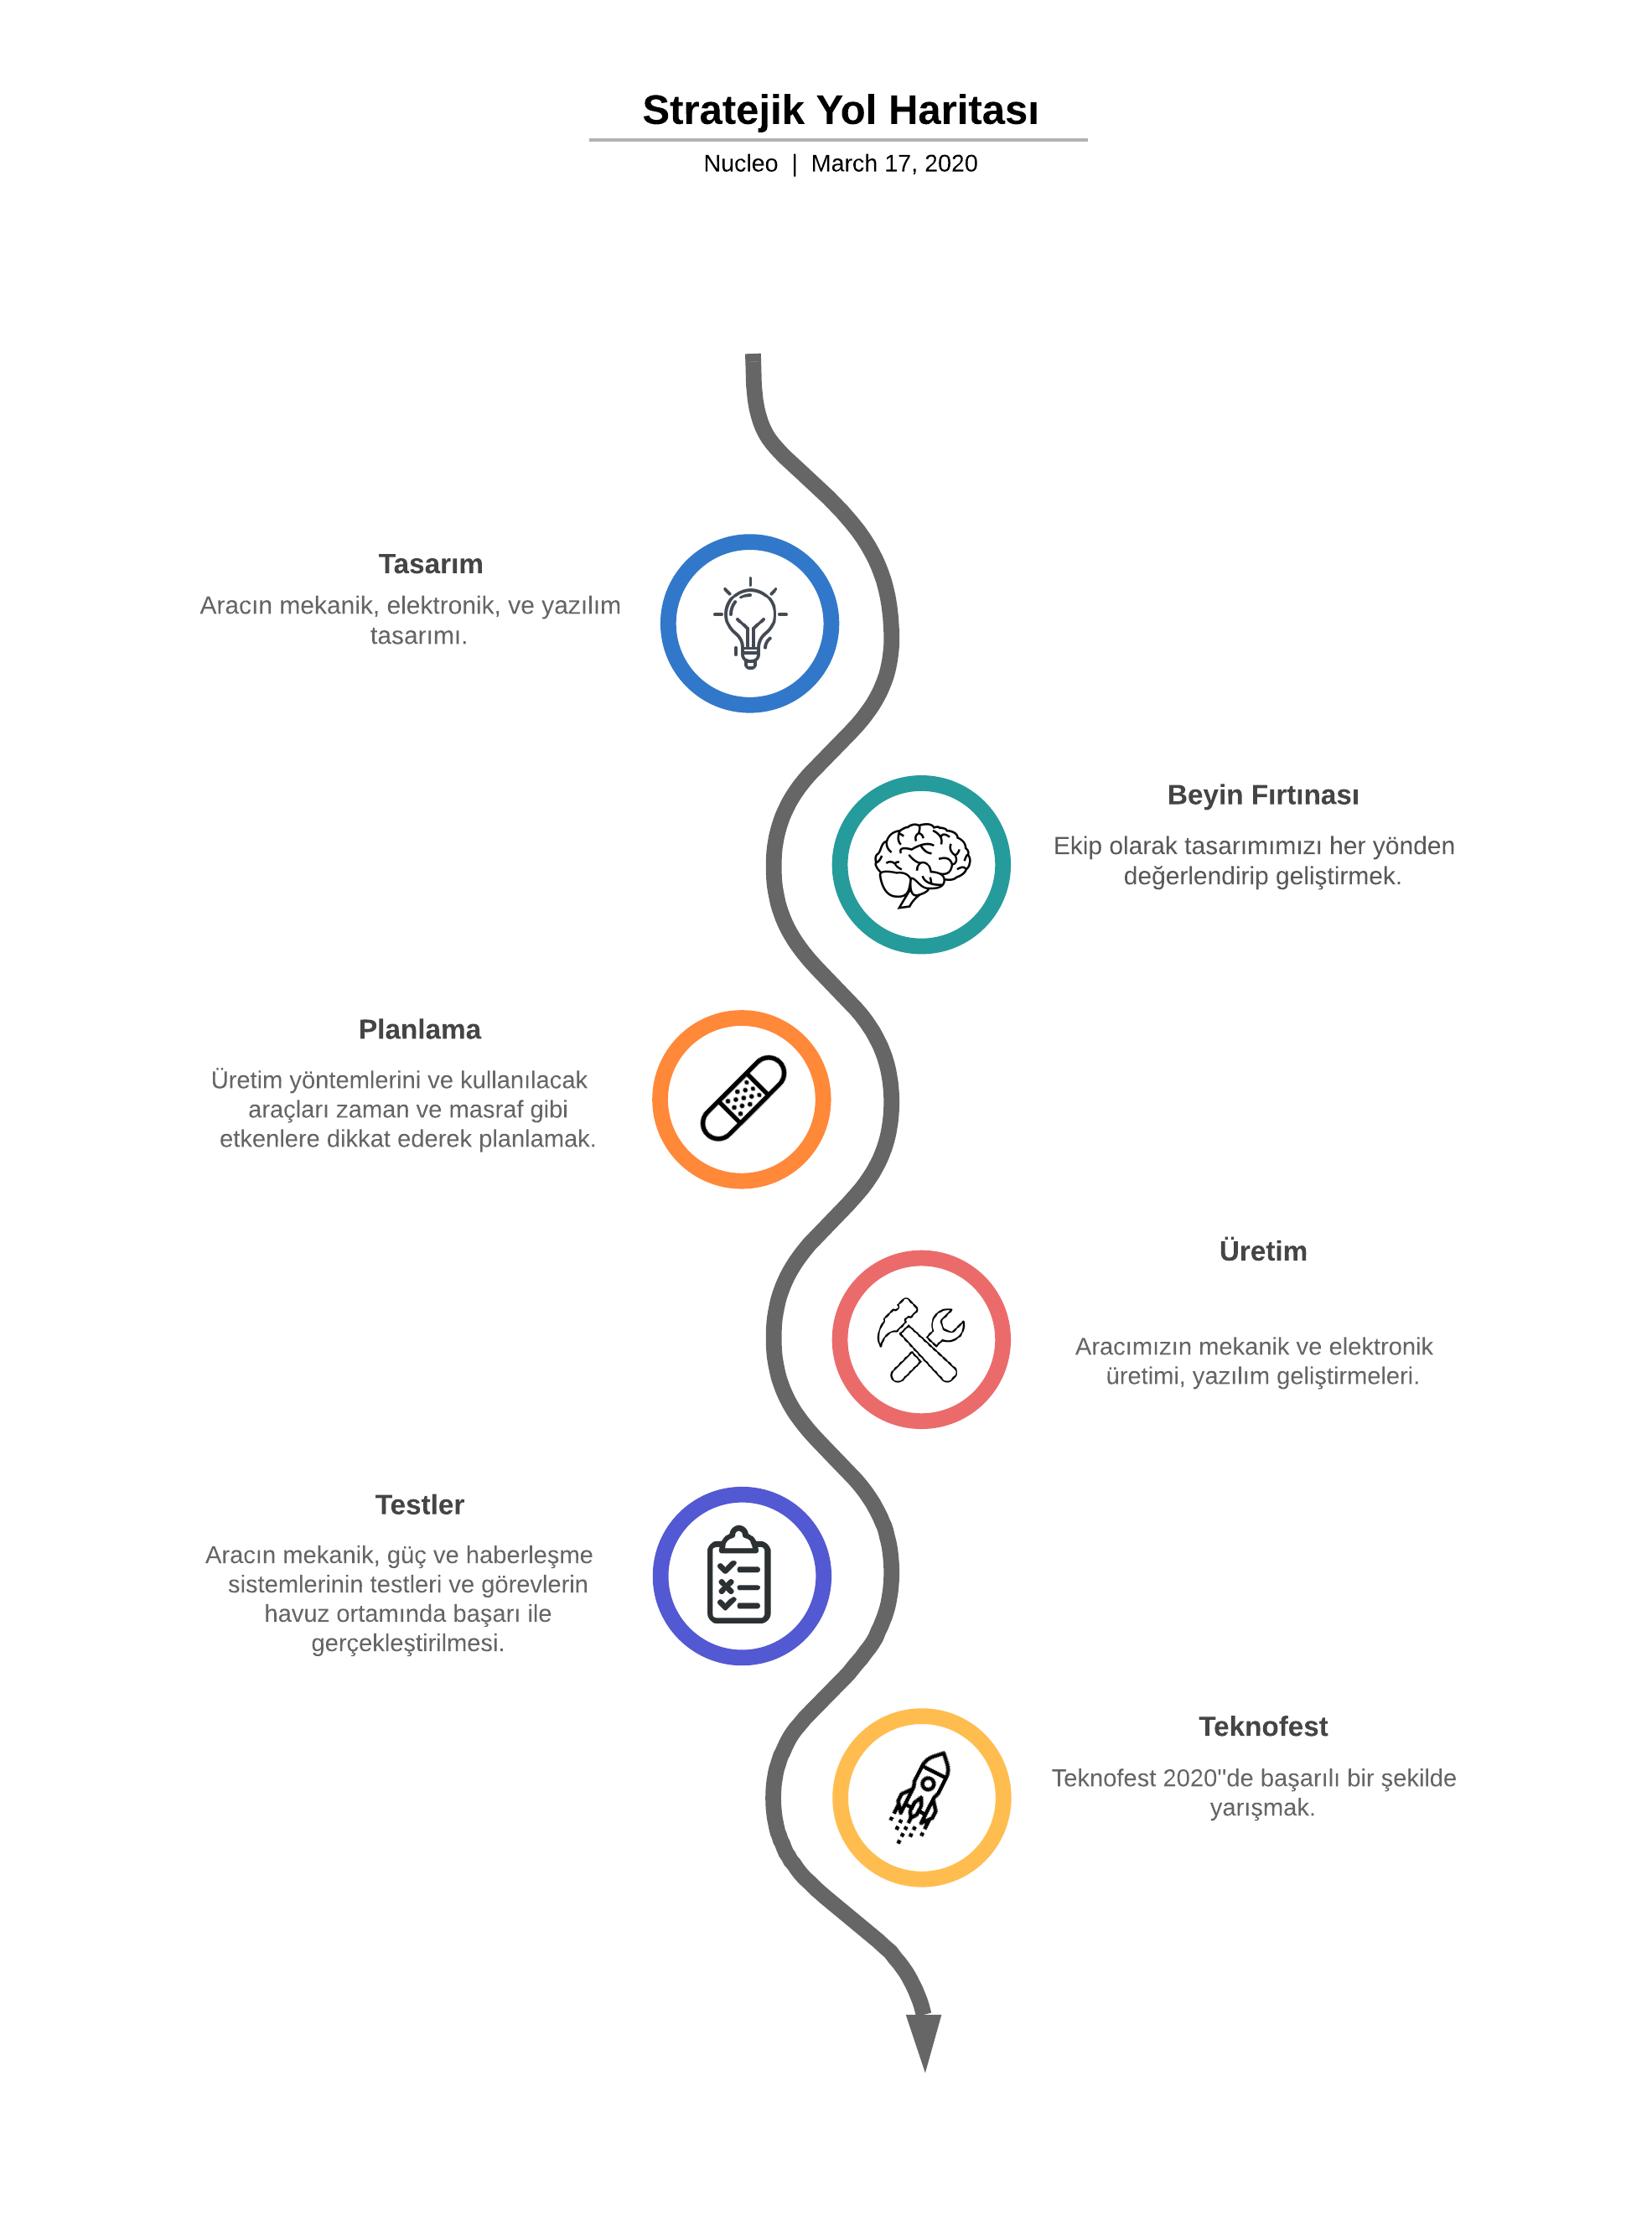
\includegraphics[width=1\textwidth]{timeline.png}
\caption{Stratejik Yol Haritası}
\label{fig:path}
\end{figure}
% Bunu organızasyon semasına mı cıkartsak?

\paragraph{} Takımımız az sayıda insandan oluşması nedeniyle, görev dağılımı yapılmış olsa da tüm üyelerin aracın her aşamasında ortak emeği olacaktır. Her üyenin bireysel olarak sorumlu olduğu görevler bulunmaktadır. Ekip üyelerimizden Enes Demirağ takımın genel organizasyonu, görüntü işleme ve haberleşme sistemleri ile, Sencer Yazıcı otonom navigasyon ve kontrolör tasarımı ile, Ege Saygılı mekanik tasarım ve üretim, Sinan Ertuğrul Yıldırım elektronik devre tasarımı ve güç sistemleri üzerinde çalışmaktadır.



\section{Araç Ön Tasarımı}

\begin{figure}[hbt!]
\centering
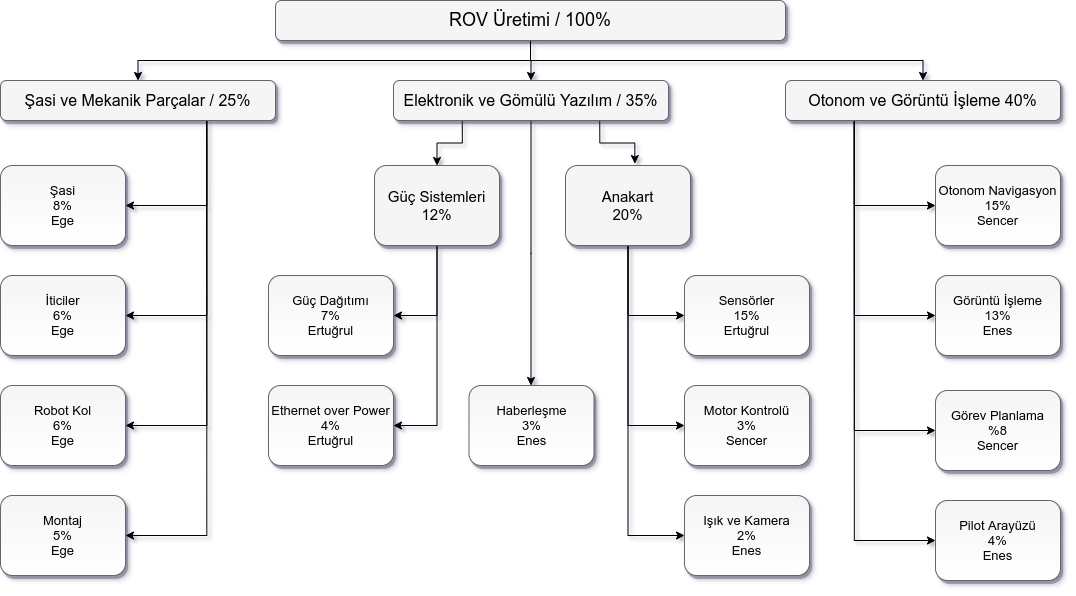
\includegraphics[width=1\textwidth]{WBS-v2.png}
\caption{İş Kırılım Yapısı(WBS)}
\label{fig:wbs}
\end{figure}

\paragraph{} Takımımızın ROV sistemi yüzeyde bulunan bir kontrol istasyonu, ve ROV'un kendisinden oluşmaktadır. Kontrol istasyonunda 15.6 inç ekrana kadar dizüstü bilgisayar kullanımı desteklenmektedir. Aynı zamanda yüzey kontrol istasyonunda 12VDC 20A kapasiteli ROV'un güç kaynağı bulunmaktadır, güç kaynağı ile ROV güç beslemesi arasında 20A bir sigorta ve acil durdurma butonu bulunmaktadır. Taşınabilir yüzey istasyonunu prize bağlanması ve ROV'unda yüzey istasyonuna bağlanmasının ardından ROV kullanıma hazır olmaktadır. Taşınabilir yüzey istayonunda aynı zamanda aracın güç ve iletişim kablosu taşınabilecektir. 

\paragraph{} ROV üzerinde beş eksende hareket özgürlüğü sağlaması için altı adet fırçasız motorlu itici bulunmaktadır. İticiler takımımız tarafından tasarlanmıştır. ROV'un elektronikleri su geçirmez akrilik bir kap içerisinde bulunmaktadır. Su geçirmez kaba kablo girişleri/çıkışları, kapak sistemleri vs. tüm su girişi olabilecek açıklıklarda o-ring conta sistemi kullanılmıştır. Aracın şasesi akrilik plastik (PMMA) malzemeden modüler bir yapıda tasarlanmıştır. Bu modülerlik sayesinde araç üzeri yapılması istenecek herhangi bir modifikasyon kolaylaştırılmıştır.
% oring a citation yapsak mi? \cite{BOOK:o-ring}

\subsection{Sistem Ön Tasarımı}
% Buraya sizce PNG yerine JPEG mi yoksak? watermark yüzünden zor okunuyor. hatta bi border bile eklenebilir. yüzey-sualtı ayrımı keskinleştirilebilir isterseniz. 
\begin{figure}[hbt!]
\centering
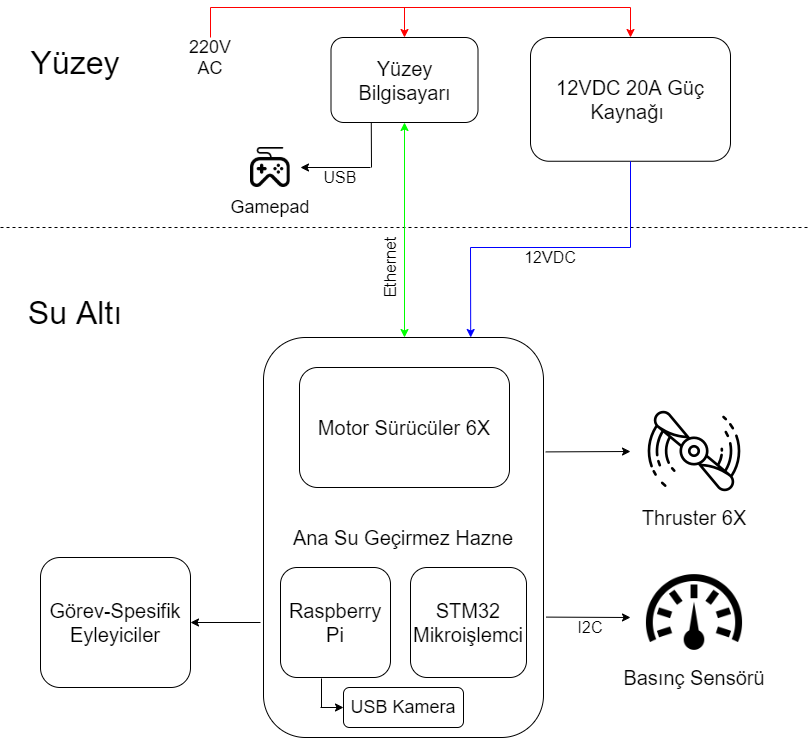
\includegraphics[width=1\textwidth]{SID.png}
\caption{Sistem Entegrasyon Diyagramı}
\label{fig:SID}
\end{figure}

\paragraph{} Sistem entegrasyon diyagramında da görüldüğü üzere, yüzey kısmında bir adet kontrol merkezi bulunmaktadır, bu taşınabilir kutu; araç kontrol bilgisayarı, araç güç kaynağı, güç kaynağı ile bağlantılı koruma(sigorta ve acil durum güç kesme butonu) vb. elemanları içerisinde barındırmaktadır. 

\paragraph{} Aracın kendisi ise, navigasyon bilgisayarı, mikroişlemci, motor sürücüler, kamera vb. elektronik elemanları içeren bir su geçirmez hazne ve suyla temas eden altı adet itici ve görev spesifik eyleyicileri içermektedir(örn. tutucu kol).

\subsection{Aracın Mekanik Tasarımı}

\subsubsection{Mekanik Tasarım Süreci}

\paragraph{} Aracın mekanik tasarımına, bütçe, malzeme erişim  ve işleme imkanları, yerli malzeme kullanımı, yarışma boy ve ağırlık sınırlamaları ve kullanılacak elektronik kontrolcülerin boyutlarından yola çıkılarak başlanmıştır. Kullanılması elzem olan elektronik komponentlerin ve o komponentlerin boyutlarının saptanmasının ardından aracın geri kalan ölçülerini belirleyecek olan ana su geçirmez haznenin boyutları belirlenmiştir. Su geçirmez hazne saydam olması, yarışma derinliği için yeterince dayanıklı olması, ucuz ve kolayca bulunabiliyor olmasından ötürü saydam akrilik tüp seçilmiştir. Ana haznenin belirlenmesinin ardından şase tasarımına geçilmiş ve haznenin şasede üst konumda bulunması amaçlanmıştır. Hazne, hacminden ötürü aracın yüzerliğinin büyük kısmını oluşturmaktadır, aracın yüzerlik merkezi ağırlık merkezine göre yukarıda ayarlanmaya çalışılmıştır, bu fark sayesinde bir düzeltme momenti oluşacak ve araç serbest halde yere parelel duracaktır, ve stabilitesi artacaktır.\cite{BOOK:rovmanual} Yüzerlik merkezi ve ağırlık merkezi arasındaki farkı daha da açmak ve ağırlık merkezini iticileri hizasına getirmek için araç su geçirmez haznesi dışında diğer tüm elemanlarını alt kısımda bulunduracak şekilde tasarlanmıştır.

% Bu resmin etrafına bi border mı eklesek acaba watermark üzerinde kötü durmuş.
\begin{figure}[hbt!]
\centering
 \begin{adjustbox}{width=7cm}
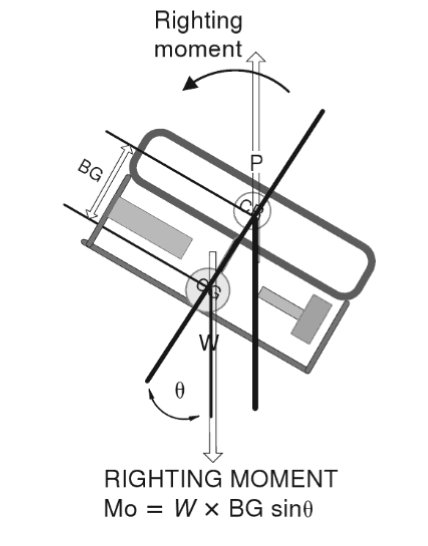
\includegraphics[width=1\textwidth]{moment.png}
 \end{adjustbox}
\caption{Düzeltme Momenti}
\label{fig:moment}
\end{figure}

\subsubsection{Malzemeler}

\paragraph{} Aracın iskeletini oluşturan parçalar ve su geçirmez haznenin tüpü gibi parçalar akrilik (PMMA) malzemeden seçilmiştir. Akrilik; hazır tüp bulunmasının kolaylığı, plaka halinde bulunmasının kolaylığı, lazer kesiminin çok kolay bulunuyor olması, ekonomik olması ve görsel özellikleri gibi sebeplerden ötürü seçilmiştir. İtici motorların koruyucu kısımları, pervaneler ve tutucu manipülatör gibi parçalar 3B plastik basım yöntemiyle üretilecektir. Su geçirmez haznenin o-ring conta bulunduran flanş parçaları alüminyumdan seçilmiştir. Araçta sabitleme elemanı olarak paslanmaz alyan başlı civatalar, paslanmaz somun ve gijonlar kullanılacaktır.

\subsubsection{Üretim Yöntemleri}

\paragraph{} Aracın şasesini oluşturan akrilik parçalar lazer kesim yöntemi ile işlenecektir. Bu yöntem ve akrilik malzeme seçimi üretim kolaylığı ve ekonomik oluşundan dolayı tercih edilmiştir. Su geçirmez kabın contalı flanşı aluminyumdan manuel torna da talaşlı imalat yöntemiyle işlenecektir. 3B plastik parçalar 3B yazıcılar yardımıyla basılacaktır.

\subsubsection{Fiziksel Özellikler}

\begin{figure}[hbt!]
\centering
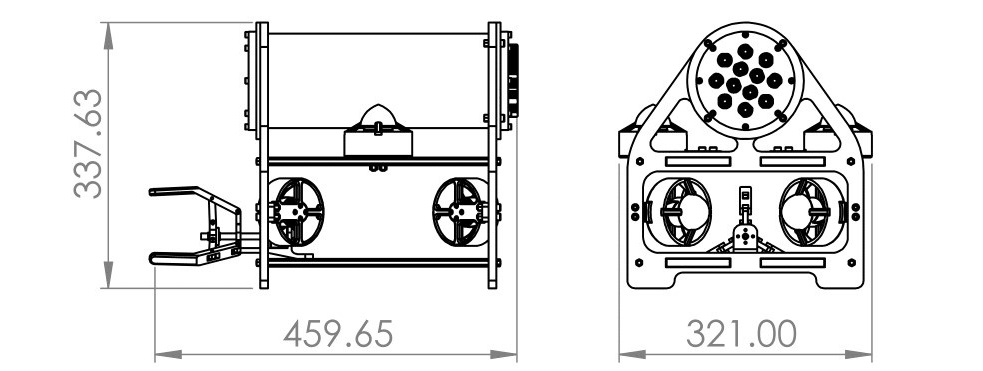
\includegraphics[width=1\linewidth]{specs.jpg}
\caption{Su Altı Aracının Ölçüleri}
\label{fig:technicaldrawing}
\end{figure}


\paragraph{} Aracın ölçüleri 32cm genişlik, 34cm yükseklik ve 46cm uzunluk şeklindedir. Aracın ağırlığı ve yüzerliği 6.8kg dır, bu sayede araç hafifçe pozitif bir yüzerliğe sahiptir, herhangi bir kontrol kaybında araç hafif yüzerliği sayesinde yüzeye çıkacak ve sudan geri alınabilecektir. 


\subsection{Elektronik, Algoritma ve Yazılım Tasarımı}

\subsubsection{Elektronik Ön Tasarım Süreci}

\paragraph{} Nucleo'nun testlerine erken başlayabilmek adına elektronik tasarımda ilk olarak temel bileşenleri barındıran ve esneklik sağlayabilecek baskı deve tasarlanmaya başlanacaktır. Anakartta önceden düşünülmüş ve kullanılacak olan güç dağıtımı, haberleşme ve sensör pinlerinin dışında yedek planlara hızlı geçiş için fazladan giriş ve çıkışlar bulundurulacaktır. İlk testlerin ardından eksik ve hatalı noktalar giderilerek devremiz güncellenecek ve bu süreç istenilen görevleri başarıyla gerçekleştirene kadar devam edecektir. 

\subsubsubsection{Enerji İletimi ve Dağıtımı}

\paragraph{} Nucleo, gücünü şebekeden gelen 220VAC gerilimi 12VDC'ye dönüştüren bir güç kaynağından alacaktır. Nucleo'nun altı motoru ve diğer elektronik devrelerinin güç gereksinimi göz önüne alındığında 30A taşıyabilecek 14AWG kablo yeterli olacaktır. Yüzey bilgisayarı ile Nucleo'nun haberleşmesi, güç kabloları üzerinden sağlanacak ve bu sayede daha az kablo kullanılacaktır. Araca aktarılan enerjinin bir kısmı doğrudan motor sürücüler ve motorlara iletilirken, bir kısmı regülatörler tarafından istenilen gerilimlere ayarlanıp ilgili bileşenlere dağıtılacaktır. Güç dağıtımı, hazırlanan güç dağıtım kartı üzerinden gerçekleştirilecektir.

\subsubsubsection{Temel Bileşenler}

\paragraph{} Nucleo'nun elektronik devreleri bir anakart ve tüp içerisindeki alanı verimli kullanabilmek adına anakart üzerine takılı yardımcı kartlardan oluşacaktır. Su altında çalışma performansı kanıtlanmış olan altı adet fırçasız doğru akım motoru, yine altı adet ESC ile sürülecektir. ESC'ler vasıtasıyla motorları kontrol edecek, görev eyleyici elemanları kontrol edecek ve gerekli sensörlerden veri alıp mikroişlemciyle haberleşerek aracın kontrolünü sağlayacak STM32F4\footnote{\href{https://www.st.com/en/microcontrollers-microprocessors/stm32f429zi.html}{https://www.st.com/en/microcontrollers-microprocessors/stm32f429zi.html}} mikrodenetleyicisi kullanılacaktır. STM32 mikrodenetleyicileri yüksek performanslı ve kullanımı kolar mikrodenetleyiciler olup, Nucleo için uygun görülmüştür. 

\paragraph{} Nucleo'nun üst seviye yazılım görevlerini gerçekleştirilebilmesi adına, yeterli performansı ile Raspberry Pi\footnote{\href{https://www.raspberrypi.org/products/raspberry-pi-3-model-b}{https://www.raspberrypi.org/products/raspberry-pi-3-model-b}} kullanılacaktır. Yüzeydeki, pilot tarafından kullanılan bilgisayar Raspberry Pi ile ethernet üzerinden haberleşecek. Pilotun istediği hareketlerin motorlar tarafından gerçekleştirilmesi Raspberry Pi'ın STM32 ile haberleşmesiyle gerçekleştirilecektir.

% Ertuğrul kanki ben iki tane footnote ekledim öylesine, bu kısım senin ben karışmıyorum istersen sil-editle-ekle sen daha iyi bilirsin.

\subsubsubsection{Yardımcı Bileşenler}

\paragraph{} Raspberry Pi tarafından işlenecek görüntü bir USB kamera vasıtasıyla alınacaktır. Nucleo'nun suyun ne kadar altında durduğunu anlaması adına bir basınç sensörü, istenilen görevleri gerçekleştirebilmesi adına bir robot kol bulunacaktır. Robot kol yine STM32 tarafından bir motor sürücü vasıtasıyla kontrol edilecektir.

\subsubsection{Algoritma Ön Tasarım Süreci}

\paragraph{} Araç uzaktan kontrol ve otonom olmak üzere iki farklı modda çalışabilecektir. Su Altı Temizlik ve Su Altı Montaj görevlerinde araç tamamen pilot kontrolünde olduğu süre boyunca kamera görüntüleri ve sensör verilerini yüzey kontrol sistemi arayüzünde görüntülerken, pilot joystick yardımıyla aracın navigasyonunu sağlayacaktır. Bunun dışında geliştirdiğimiz PID kontrolör sayesinde araç pilot müdahale etmediği sürecek bulunduğu son derinliği koruyacaktır.

\paragraph{} Engel Geçiş ve Denizaltı Tespit görevleri pilot müdahalesi olmadan tamamen otonom olarak hareket edecektir. Görüntü işleme algoritmamız ile göreve yönelik hedefler tespit edilecek ve güdüm kontrolü ile su altı navigasyon sağlanacatır. Bu süre içerisinde yer istasyonu ile olan uzaktan kontrol sistemi pasif duruma geçecek ve gözlem amaçlı olarak tek yönlü bir şekilde kamera görüntüleri ve sensör verileri yüzeye aktarılacaktır.

\begin{figure}[hbt!]
\centering
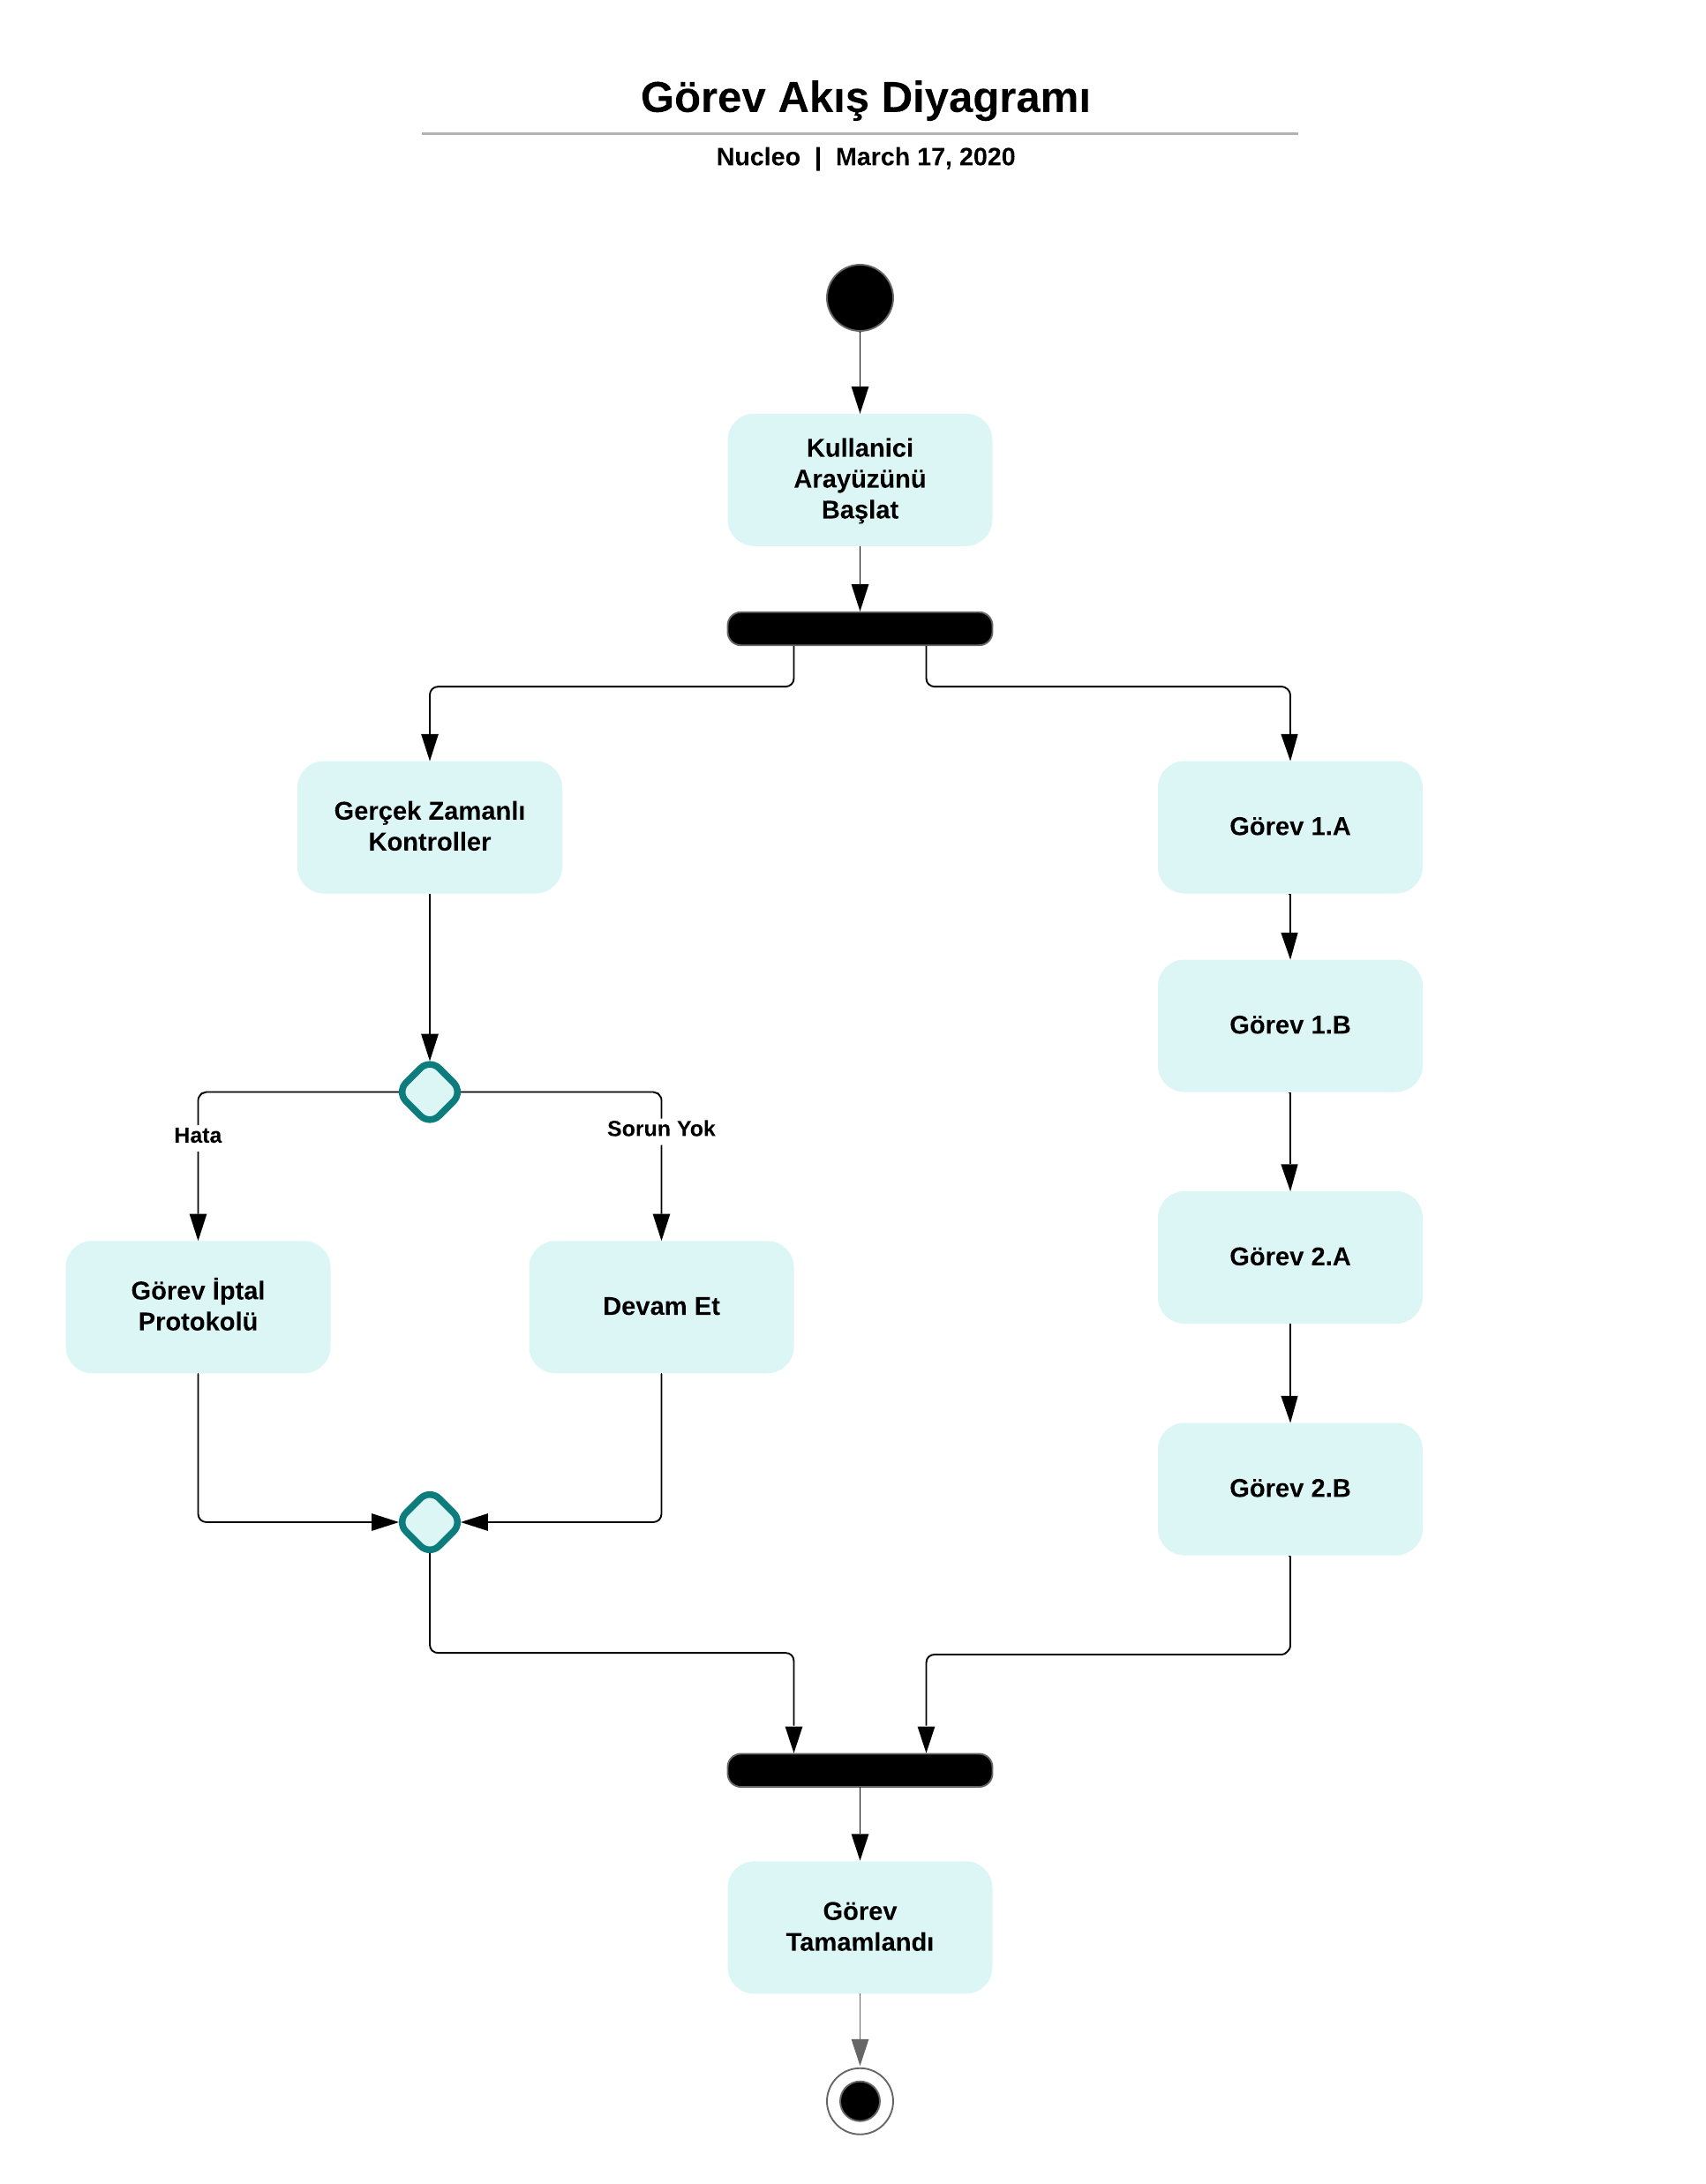
\includegraphics[width=1\textwidth]{akis-diyagrami.png}
\caption{Akış Diyagramı}
\label{fig:flow-chart}
\end{figure}


\subsubsection{Yazılım Ön Tasarım Süreci}


\paragraph{} Yazılım ekibi üyemiz Sencer Yazıcı, aynı zamanda İTÜ AUV Takımı yazılım ekip liderliğini üstlendiğinden, İTÜ AUV Takımı bünyesinde geliştirilen yazılımı kullanmayı hedeflemekteyiz. Takımda geliştirilen yazılım, modüler bir altyapı içerdiğinden, kolayca entegre edilebilecektir.

\paragraph{} Başlıca sistemi genel parçalara ayıracak olursak
\begin{itemize}
    \item STM32F429ZI Mikrokontrolör üzerinde çalışacak olan gömülü sistem, alt seviye yazılım
    \item Raspberry Pi Üzerinde çalışacak olan, karar verme mekanizmasına ve haberleşme sistemlerine sahip sistem, üst seviye yazılım
    \item Yer istasyonunda çalışacak olan, operatör komutlarının aracın komuta sistemine aktarılmasını sağlayan haberleşme çift yönlü telemetri (veri aktarımı)
\end{itemize}

\subsubsubsection{Gömülü Sistem \& Mikrokontrolör}

 \paragraph{}  Anakart üzerine takılı STM32F429ZI mikrokontrolörün, temel görevi alt seviye elektronik işlemleri ve aracın temel fonksiyonlarını kontrol etmektir. Geliştirilen gömülü yazılım, güç hattının gerilimini hassas bir şekilde ölçerek motorları istenilen kuvveti üretecek şekilde bir PWM sinyali üretir. Burada, ekibimiz tarafından motorun su altında yapılan testleriyle elde edilen PWM - Kuvvet karakteristiği kullanılır. bu sayede test edilen gerilim aralığında herhangi bir gerilimde, mikrokontrolör istenilen kuvveti üretecek PWM sinyaini hesaplayabilir, ve böylece 5-Eksen PID kontrolör ile kontrol sistemi çalıştırılır. Burada SimScape üzerinde yapılan CFD testleri ile de, drag (direnç) ve damping (sönüm) katsayıları hesaplanır. Bu hesaplar sonucu elde edilen matematik modele göre bir PID kontrolör tasarlanır, ve su altında gerçek sistem üzerinde yapılan testler sonucu ince ayar (Fine Tuning) yapılarak nihai parametrelere ulaşılır. 

\paragraph{} Ayrıca gömülü sistem, basınç sensöründen elde ettiği veriyi, Kalman Filtresi ile filtreleyerek 5 eksen kontrol sisteminde kullanılacak olan derinlik geribeslemesini hesaplar.

%%%%%% BURAYA BI KALMAN FITRESI CITATION GUZEL GIDER %%%%%% kanka çok gerekli değilse yapmasak mı ? çünkü verdiğimiz citation bi anlam ifade etmezse boşuna koymuş olmayalım. ama araştıralım uygun bişey bulursak koyalım. koymuş olmak için koymayalım yani bence


\paragraph{} Bunun yanı sıra, yine temel fonksiyonlar kategorisine giren, eyleyicilerin (manipülatörlerin) kontrolünü de, gömülü yazılım yürütür.

\paragraph{} Son olaraksa, tüm bu verilerin ve kontrol sistemlerinin, temel karar verme mekanizmasının bulunduğu ana bilgisayara iletilmesi içinse, istenirse Ethernet, isternirse UART kullanılabilir. Gömülü sistem bu iletişim yöntemlerinin hangisinin aktif olduğunu belirleyerek birinden ötekine dinamik olarak geçebilmektedir. Gömülü yazılım tüm bunları, ROS\footnote{\href{https://www.ros.org}{https://www.ros.org}} topic ağı üzerinde gerçekleştirmekte olup, herhangi bir topic'i dinleyebilir, herhangi bir topic'e veri aktarımı yapabilmektedir. 

%%%%%% BURAYA ROS SİTESİNE Bİ FOOTNOTE GUZEL GIDER %%%%%% koydum bir tane generic link (değiştirilebilir) 

\paragraph{} Bu gömülü sistem, yazılım ekibi üyemiz tarafından İTÜ AUV Takımı bünyesinde geliştirilmiştir ve tamamen özgündür. Bu yazılım İTÜ AUV Takımında da aktif olarak kullanılmaktadır ve modüler yapısı sayesinde teknofest yarışması için de kolayca entegre edilebilecektir.  
% todo: topic nedir hacım ? xD


\subsubsubsection{Merkezi Bilgisayar ve Karar Mekanizması Sistemi}

\paragraph{} Aracın temel fonksiyonları gömülü yazılım tarafından STM32 üzerinde gerçekleştirilirken, görev akışını ve üst seviye hesaplamaları gerçekleştirecek olan bilgisayar, Raspberry Pi 2, Ethernet ve ya UART üzerinden STM32 ile haberleşerek temel fonksiyonların üst seviye yazılımlar ile iletişimini sağlar. Üst seviye yazılımlarda, ROS ağı üzerinde çalışacak olan yazılımlar, görüntü işleme ve HD USB Kamera görüntüsünün yüzeye aktarılması bulunur.

\paragraph{} ROS ağı üzerinde bulunan Node'lar, temel olarak veri iletişimi, acil durum kontrolü, görüntü işleme sonucu elde edilen verileri işleme ve gerekli durumlarda tespit edilen objelerin pozisyon ve oryantasyon tespiti (tahmini) ve bu pozisyon(lar)ın filtrelenmesi gibi konuları gerçekleştirir.

% Bir subsubsubsection da ben yaziyorum kanki goruntu isleme ile ilgili
\subsubsubsection{Görüntü İşleme}
\paragraph{} Araç üzerindeki kameralardan alınan görüntü Raspberry Pi üzerinde çalışan bir Python programı ile işlenip analiz edilerek, araca otonom olarak görev odaklı komutlar verilecektir. Görüntü işleme sisteminde openCV kütüphanesi kullanılacaktır. Elde edilen kamera görüntüsü su altında optimize edilecek görüntü işleme filtrelerinden\cite{ARTICLE:image_proc} geçirilecek ve geliştirdiğimiz görev karar algoritması sonucu yüzey kontrol istasyonundan tamamen bağımsız olarak, otonom bir şekilde görevleri gerçekleştirecektir.


\begin{figure}
\centering
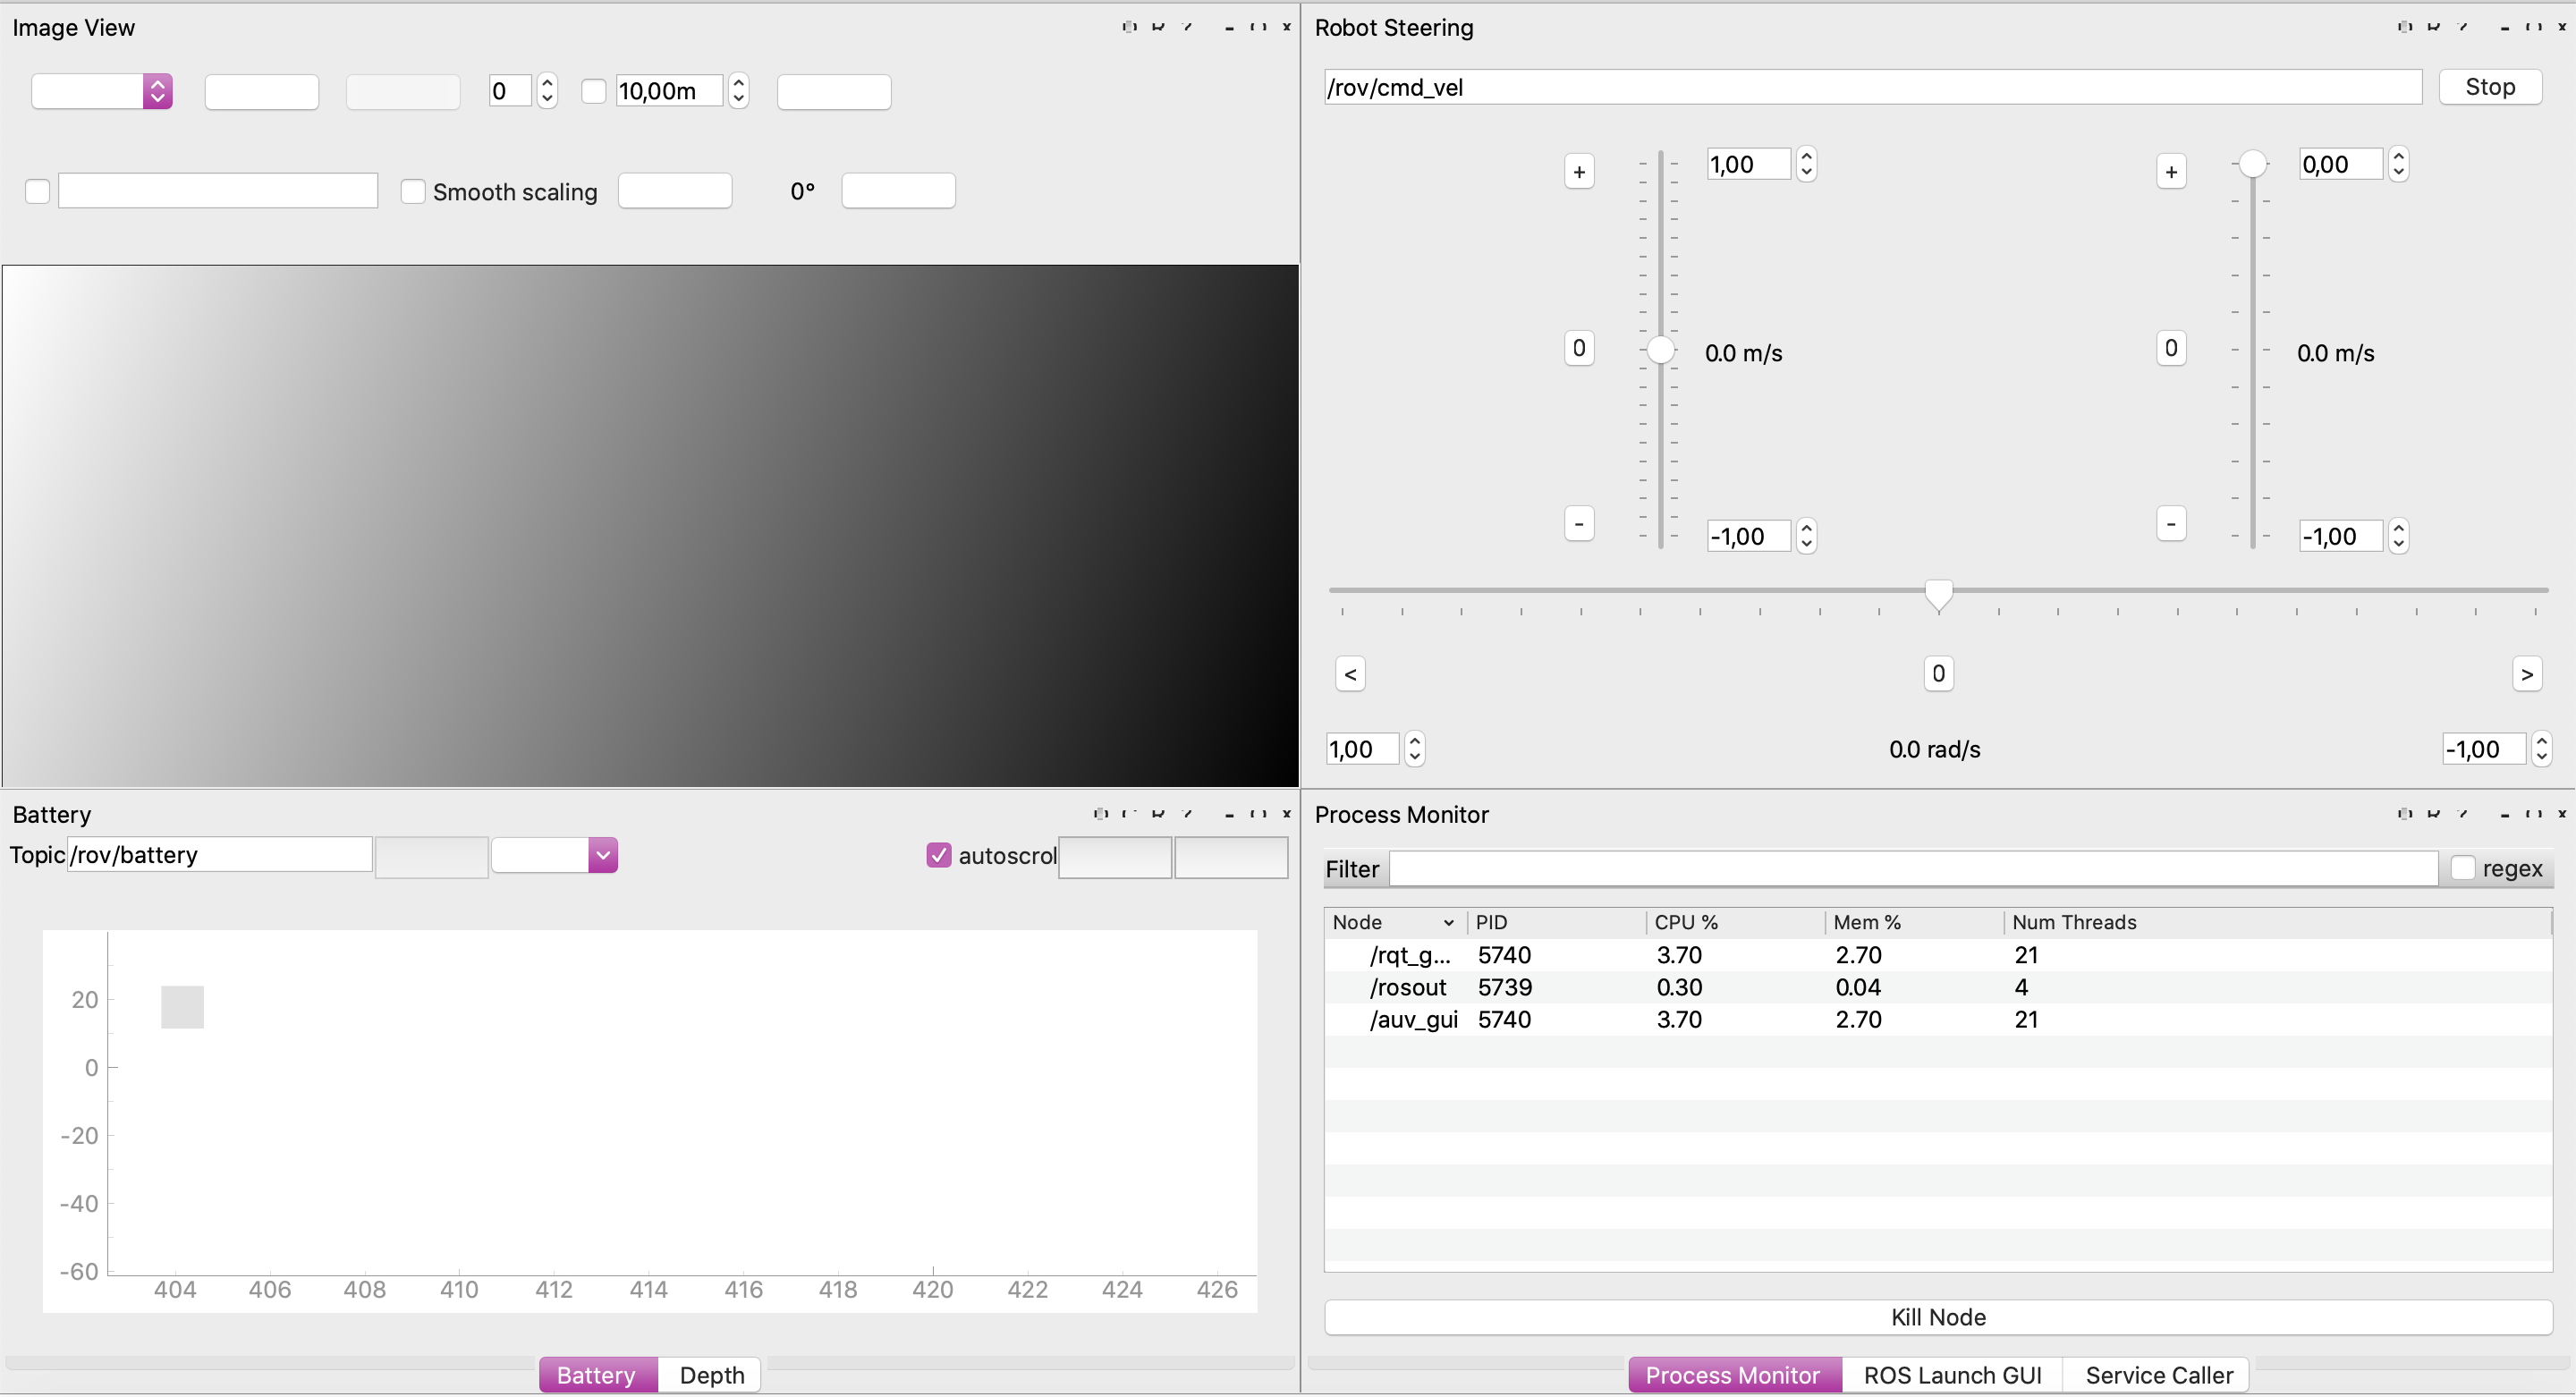
\includegraphics[width=1\textwidth]{gui.png}
\caption{Örnek bir GUI}
\label{fig:gui}
\end{figure}
\subsubsection{GUI} % bunu üste almak gerekmez mi?
% GUI ile Dıs arayüz aynı şey mi? eğer öyleyse Dış Arayüz (GUI) yazalım mı başlığa hem türkçeye daha uygun hem örnek raporda öyle.
\paragraph{} ROS ağının TCP/IP üzerinden çalışıyor olmasının avantajlarından faydalanarak, Rqt tabanlı bir GUI geliştirmeyi düşünmekteyiz. Bu sayede yüzeydeki bilgisayar, Raspberry Pi'ın IP adresi ile, 11311 numaralı porttan ROS ağına bağlanabilecek ve ROS ağı üzerindeki tüm topic'leri dinleyebilecek ve ya bu topic'lere veri aktarabilecektir. İTÜ AUV Takımı için oluşturmuş olduğumuz örnek bir GUI Şekil \ref{fig:gui}'de verilmiştir.

%%%%%% BAZI YERLERDE "Pilot Arayüzü" BAZI YERLERDE "GUI" BAZI YERLERDE "Yer İstasyonu" BAZI YERLERDE "Kontrol İstasyonu" denilmiş. Bunlarda neyi kastettiğimize göre belirtip, düzeltelim.


\section{Güvenlik}


\paragraph{} Aracımızın tasarımı gibi teknik, üretim ve montaj gibi pratik işlerin yanısıra en büyük önceliğimiz iş güvenliği ve emniyetdir. Testlerde, atölye çalışmalarında, önceliğimiz çalışmak için güvenli ve konforlu alanı oluşturmak olacaktır. Takım olarak, ekip üyelerine herhangi bir zarar gelmemesi ve olası iş kazalarını önlemek için her türlü önlemi uygulamaktan çekinmeyeceğiz.
Atölye çalışmalarımızda kişisel koruyucu ekipmanlar olan gözlük, eldiven, maske gibi ekipmanların kullanılmasının yanında atölyemizde acil göz banyosu ve ilk yardım kiti bulundurmayı da ihmal etmeyeceğiz.

\paragraph{} Aracımızın teknik özelliklerine dikkat ederken, güvenlik önlemlerini de göz ardı etmedik. Aracın üzerindeki motorların yerleşimi dışarıdan zarar gelmeyecek ve dışarıya zarar vermeyecek şekilde konumlandırıldı. Bunların yanında, aracın üzerinde kullanılacak tüm plastik kelepçeler kullanıcılara zarar veremeyecek şekilde tıraşlanacak ve aracın üzerinde hiçbir sivri yüzey bırakılmayacaktır. Aracın su altında herhangi bir sorunda karşılaşılması durumunda yer istasyonunda bulunan acil durdurma butonu sayesinde aracı hızlı bir şekilde durdurabilme imkanımız bulunmaktadır. Ayrıca güç hesaplamaları yapılacak ve dağıtım hatlarında uygun sigortalar ve koruma devreleri kullanılacaktır.
% Sızdırmazlık ve kabloların yalıtımı hakkında bısıyler eklenebılır.
% Motorlarımızın sualtına uygun potlanacagını ve korozyondan korunacagını yazabılırız.

\section{Zaman, Bütçe ve Risk Planlaması}
\subsubsection{Zaman Planlaması}
\paragraph{} Blablabla
\begin{figure}[hbt!]
\centering
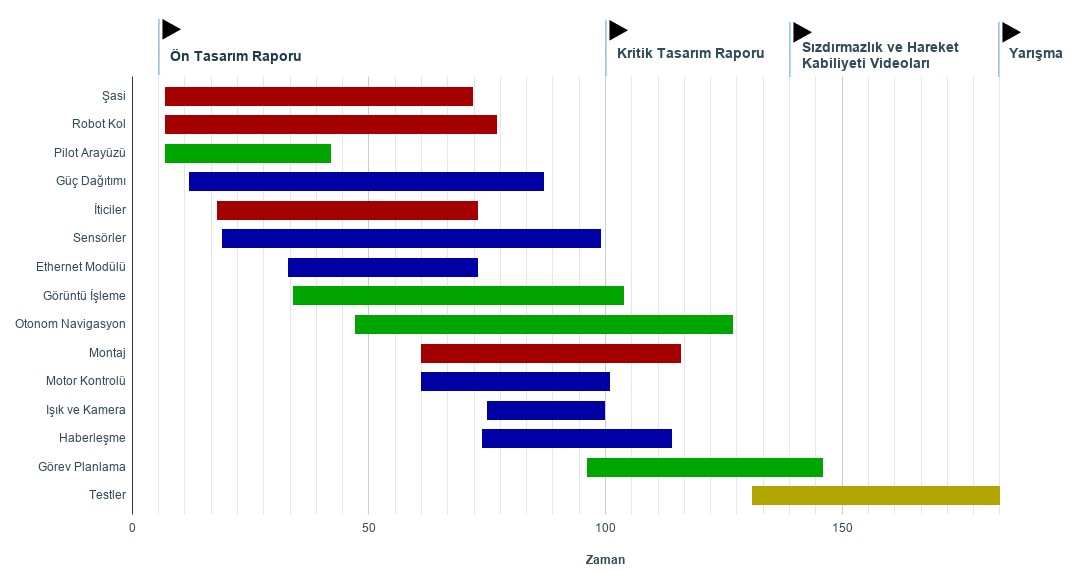
\includegraphics[width=1\textwidth]{chart-final.png}
\caption{Zaman Çizelgesi}
\label{fig:gantt-chart}
\end{figure}

\subsubsection{Bütçe Planlaması}
% Buraya butce gelecek ama Sekil degil Tablo yazsin altinda. 
\begin{figure}[hbt!]
\centering
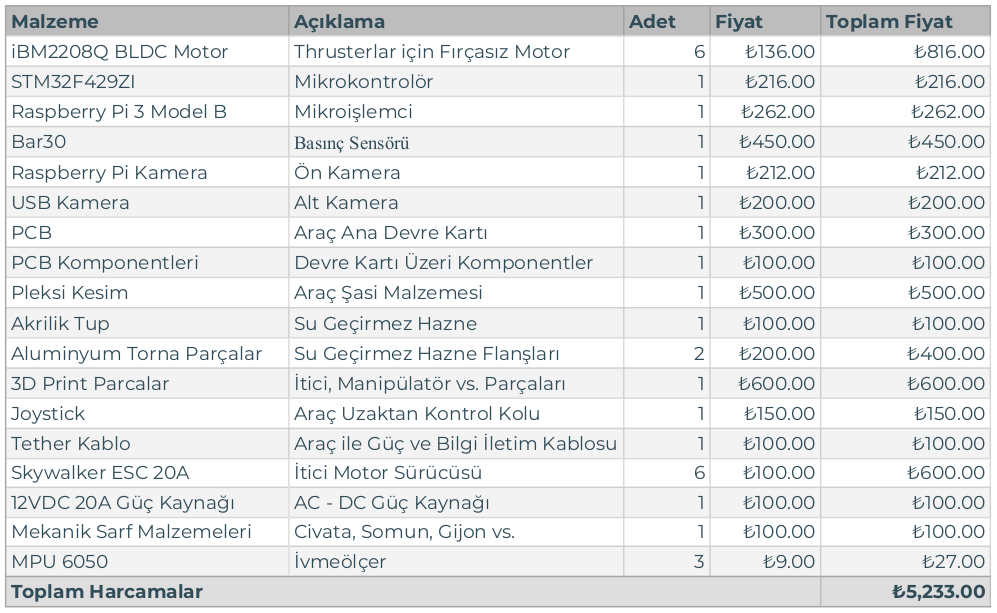
\includegraphics[width=1\textwidth]{butce.png}
\caption{Bütçe}
\label{fig:butce}
\end{figure}

\subsubsection{Risk Planlaması}

\paragraph{} Riskler aşağıda belirtilmiştir, ancak bu alandaki tecrübelerimizin yardımıyla projeyi başarıyla tamamlayacağımıza eminiz.

\begin{itemize}
    \item Coronavirus nedeniyle proje planlanandan daha uzun sürebilir.
    \item Yurtdışı malzeme temininde yaşanacak sıkıntılara alternatif çözüm aramak gerekebilir.
    \item Projenin beklenenden daha maliyetli olması ekonomik sorunlara neden olabilir.
\end{itemize}

\section{Özgünlük}

\paragraph{} Ozgunluk hakkinda her alandan birer cumle ile bir paragraf yazilacak.
1 - Qground yerine kendi customizable GUImiz var
2 - Pixhawk yerine kendi kontrolorumuz var
3 - Kendi iticilerimizi tasarlayıp, üretip potlayacağız. T100/200 kullanmayacağız. Aynı kalitede daha ucuza yerli üreteceğiz.




\newpage
\section{Referanslar}
\vspace{-1cm}
\printbibliography[title={\textbf{ }}]


\end{document}
